% ============================================================
%  Slide template -- Tối ưu hóa Pipe trong xv6
%  Compile: latexmk -r latexmkrc main.tex   (XeLaTeX)
% ============================================================
\documentclass[aspectratio=169]{beamer}

%% ----- Encoding / Language -----
\usepackage{fontspec}
\defaultfontfeatures{Ligatures=TeX}
\usepackage[vietnamese]{babel}

%% ----- Math -----
\usepackage{amsmath, amssymb, mathtools}
\usefonttheme{professionalfonts}

%% ----- Tables -----
\usepackage{booktabs}
\usepackage{multirow}
\usepackage{tabularx}

%% ----- Code listings -----
\usepackage{listings}
\lstset{
    language=C,
    basicstyle=\ttfamily\small,
    keywordstyle=\color{blue!80!black}\bfseries,
    commentstyle=\color{gray},
    stringstyle=\color{orange!80!black},
    breaklines=true,
    frame=single,
    rulecolor=\color{gray!30},
    backgroundcolor=\color{gray!5},
    showstringspaces=false,
}

%% ----- Custom macros (highlight, bracket shortcuts, etc.) -----
\usepackage{mymacro}

%% ----- Beamer theme -----
\usetheme{default}
\usecolortheme{default}

% Color palette
\definecolor{bkhnblue}{RGB}{0,84,166}
\definecolor{bkhnlight}{RGB}{220,235,255}

\setbeamercolor{frametitle}{fg=white, bg=bkhnblue}
\setbeamercolor{title}{fg=bkhnblue}
\setbeamercolor{subtitle}{fg=bkhnblue!70!black}
\setbeamercolor{author}{fg=black}
\setbeamercolor{date}{fg=black!60}
\setbeamercolor{structure}{fg=bkhnblue}
\setbeamercolor{block title}{fg=white, bg=bkhnblue}
\setbeamercolor{block body}{bg=bkhnlight}
\setbeamercolor{alerted text}{fg=red!80!black}

\setbeamerfont{frametitle}{series=\bfseries, size=\large}
\setbeamertemplate{navigation symbols}{}

\setbeamertemplate{footline}{%
    \raisebox{8pt}{%
        \makebox[\paperwidth]{%
            \hfill
            \makebox[5em]{\footnotesize\textcolor{gray!70}{\insertframenumber/\inserttotalframenumber}}%
        }%
    }%
}

\setbeamertemplate{itemize item}{\color{bkhnblue}$\blacktriangleright$}
\setbeamertemplate{itemize subitem}{\color{bkhnblue!60}$\triangleright$}

%% ----- Title info -----
\title{Tối ưu hóa Pipe để Cải thiện\\Thông lượng IPC trong xv6}
\subtitle{Mã dự án: 25236}
\author{Nguyễn Sỹ Tuấn \and Lê Huy Sơn \and Vũ Tiến Long}
\institute{Trường Điện -- Điện tử · Đại học Bách Khoa Hà Nội}
\date{Hệ điều hành [Multimedia] -- 20252}

% ============================================================
\begin{document}

%% --- Title slide ---
\begin{frame}[plain]
    \maketitle
\end{frame}

%% --- Work distribution ---
\begin{frame}{Phân công công việc \& Đóng góp}
    \renewcommand{\arraystretch}{1.18}
    \footnotesize
    \begin{tabularx}{\linewidth}{|c|p{2.5cm}|X|c|}
        \hline
        \textbf{STT} & \textbf{Thành viên} & \textbf{Nội dung công việc} & \textbf{\%} \\
        \hline
        1  & \multirow{4}{*}{\centering\textbf{Nguyễn Sỹ Tuấn}}
           & v2 -- Bulk Copy                                       & 15\% \\
        \cline{1-1}\cline{3-4}
        2  & & v4 -- Multi-page Allocation                         & 15\% \\
        \cline{1-1}\cline{3-4}
        4  & & Baseline v1, viết \texttt{pipebench.c} và báo cáo  &  4\% \\
        \hline
        5  & \multirow{3}{*}{\centering\textbf{Lê Huy Sơn}}
           & v3 -- Ring of Buffers                                 & 15\% \\
        \cline{1-1}\cline{3-4}
        6  & & v6 -- Priority Boost                                & 15\% \\
        \cline{1-1}\cline{3-4}
        7  & & v8 -- All Combined (tích hợp v3, v6)               & 3\% \\
        \hline
        8  & \multirow{3}{*}{\centering\textbf{Vũ Tiến Long}}
           & v5 -- Lazy Wakeup                                     & 15\% \\
        \cline{1-1}\cline{3-4}
        9  & & v7 -- Cache-line Alignment                          & 15\% \\
        \cline{1-1}\cline{3-4}
        10 & & v8 -- All Combined (tích hợp v5, v7)               &  3\% \\
        \hline
        \multicolumn{3}{|c|}{\textbf{Tổng}} & \textbf{100\%} \\
        \hline
    \end{tabularx}
    \renewcommand{\arraystretch}{1}
\end{frame}

%% --- Table of contents ---
\begin{frame}{Nội dung}
    \tableofcontents
\end{frame}

% ============================================================
\section{Giới thiệu}
% ============================================================

\begin{frame}{Pipe trong UNIX/xv6}
    \begin{columns}[c]
        \begin{column}{0.54\textwidth}
            \begin{itemize}
                \item Pipe là cơ chế IPC \textbf{unidirectional, half-duplex}
                \item Hiện thực dưới dạng \textbf{bounded buffer} trong kernel
                \item Hai đầu: \texttt{fd[0]} (đọc) và \texttt{fd[1]} (ghi)
                \item Dữ liệu hoàn toàn trên RAM, không qua đĩa
            \end{itemize}
            \vspace{0.5em}
            Pipe được minh họa theo cơ chế \textbf{Producer-Consumer Problem}
            (Dijkstra, 1965): tiến trình ghi đóng vai \emph{Producer},
            tiến trình đọc đóng vai \emph{Consumer}, bộ đệm vòng là
            \emph{Buffer} dùng chung.
        \end{column}
        \begin{column}{0.43\textwidth}
            \centering
            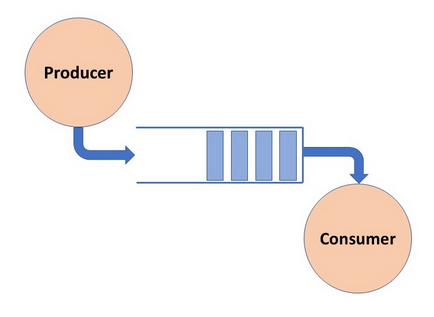
\includegraphics[width=\textwidth]{../figures/ProCon.png}
        \end{column}
    \end{columns}
\end{frame}

\begin{frame}{Công thức tính băng thông}
    \begin{equation*}
        \text{Throughput (B/s)}
        = \frac{\text{total\_bytes}}{\text{time (s)}}
        = \frac{\text{total\_bytes} \times \text{TICKS\_PER\_SEC}}{\text{elapsed\_ticks}}
    \end{equation*}

    \vspace{0.6em}
    \begin{itemize}\setlength\itemsep{6pt}
        \item \textbf{total\_bytes}: tổng số byte cần truyền qua pipe
        \item \textbf{TICKS\_PER\_SEC}: số tick trong 1 giây (xv6: timer interrupt tăng tick, $\approx 10$ tick/s)
        \item \textbf{elapsed\_ticks}: thời gian truyền hết dữ liệu tính bằng tick (\texttt{uptime()} syscall)
    \end{itemize}

    \vspace{0.6em}
    Đơn vị đo: \textbf{B/s} (hoặc KB/s, MB/s). Trong báo cáo dùng $1\,\text{MB/s} = 2^{20}\,\text{B/s}$.
\end{frame}

\begin{frame}[fragile]{Cấu trúc các trường trong \texttt{struct pipe}}
    \begin{columns}[c]
        \begin{column}{0.44\textwidth}
            \begin{lstlisting}
#define PIPESIZE 512

struct pipe {
  struct spinlock lock;
  char   data[PIPESIZE];
  uint   nread;
  uint   nwrite;
  int    readopen;
  int    writeopen;
};
            \end{lstlisting}
        \end{column}
        \begin{column}{0.53\textwidth}
            \begin{itemize}\setlength\itemsep{6pt}
                \item \textbf{lock} -- spinlock bảo vệ toàn bộ struct, ngăn race condition
                \item \textbf{data[]} -- bộ đệm vòng 512 byte
                \item \textbf{nread, nwrite} -- chỉ số tích lũy (không reset):
                    \begin{itemize}\setlength\itemsep{2pt}
                        \item Đầy: \texttt{nwrite == nread + PIPESIZE}
                        \item Rỗng: \texttt{nread == nwrite}
                        \item Truy cập: \texttt{data[nwrite \% PIPESIZE]}
                    \end{itemize}
                \item \textbf{readopen, writeopen} -- cờ báo đầu pipe còn mở
            \end{itemize}
        \end{column}
    \end{columns}
\end{frame}

\begin{frame}{Các hàm cơ bản trong \texttt{pipe.c}}
    \begin{itemize}\setlength\itemsep{10pt}
        \item \textbf{pipealloc():} cấp 1 trang cho pipe và tạo 2 file descriptor \texttt{f0}, \texttt{f1} để đọc và ghi
        \item \textbf{pipewrite():} ghi dữ liệu từ user space vào bộ đệm vòng; nếu buffer đầy thì \texttt{sleep} chờ reader
        \item \textbf{piperead():} đọc dữ liệu từ bộ đệm vòng ra user space; nếu buffer rỗng thì \texttt{sleep} chờ writer
        \item \textbf{pipeclose():} đóng một đầu pipe, đánh thức bên đối diện; giải phóng bộ nhớ khi cả hai đầu đã đóng
    \end{itemize}
\end{frame}

\begin{frame}{Các yếu tố tác động đến băng thông}
    \begin{itemize}\setlength\itemsep{8pt}
        \item \textbf{Chi phí gọi syscall:}
        \item \textbf{Kích thước pipe buffer:} PIPESIZE = 512 B quá nhỏ.
        \item \textbf{copyin/copyout:} copy từng byte một thay vì copy nhiều byte mỗi lần.
        \item \textbf{Spinlock \& sleep/wakeup:} \texttt{wakeup()} vô điều kiện phải quét toàn bộ \texttt{proc[]} mỗi lần ghi.
        \item \textbf{Scheduler:} không ưu tiên reader/writer khi pipe có dữ liệu.
        \item \textbf{CPU cache -- False sharing:} \texttt{nread} và \texttt{nwrite} cùng cache line khiến CPU invalidate cache liên tục trên SMP
    \end{itemize}
\end{frame}


% ============================================================
\section{Các phiên bản tối ưu}
% ============================================================

\begin{frame}{Nhận xét về \texttt{chunk\_bytes}}
    \begin{itemize}\setlength\itemsep{10pt}
        \item \texttt{chunk\_bytes} càng lớn thì số lần gọi syscall càng ít, giúp giảm overhead trap vào kernel
        \item Số lần gọi syscall $=$ \texttt{total\_bytes} $/$ \texttt{chunk\_bytes} -- chunk nhỏ $\Rightarrow$ băng thông bị giới hạn bởi chi phí syscall
        \item Tuy nhiên chunk lớn hơn đồng nghĩa mỗi lần \texttt{write()} phải chờ reader drain buffer nhiều lần hơn, làm tăng chi phí \texttt{sleep()}/\texttt{wakeup()}
        \item Đây là sự \textbf{đánh đổi} giữa ít syscall và nhiều lần chờ đồng bộ
        \item Đo băng thông với \texttt{chunk\_bytes} = 64, 128, 256, 512, 1024, 2048, 4096 để thấy rõ sự thay đổi
    \end{itemize}
\end{frame}


\begin{frame}[fragile]{v2 -- Bulk Copy}
    \textbf{Giải quyết vấn đề:}
    \begin{itemize}
        \item v1 gọi \texttt{copyin()/copyout()} từng byte một $\Rightarrow$ $n$ lần cho $n$ byte
    \end{itemize}

    \vspace{0.4em}
    \textbf{Cách giải quyết:}
    \begin{itemize}\setlength\itemsep{3pt}
        \item Ghi/đọc cả khối \texttt{chunk\_bytes} trong một lần \texttt{copyin()}
        \item Tính số byte có thể copy an toàn: \texttt{min(còn\_lại, free\_slots, till\_wrap)}
        \item Số lần \texttt{copyin()} giảm từ $n$ xuống $\lceil n / \texttt{chunk\_bytes} \rceil$
    \end{itemize}

    \vspace{0.4em}
    \textbf{Source code thay đổi:}
\begin{lstlisting}
int to_copy = min(n-i, free_slots, till_wrap);
copyin(pr->pagetable, &pi->data[head_slot], addr+i, to_copy);
pi->nwrite += to_copy;
\end{lstlisting}
\end{frame}

\begin{frame}[fragile]{v3 -- Ring of Buffers}
    \textbf{Giải quyết vấn đề:}
    \begin{itemize}
        \item v2 vẫn bị giới hạn bởi PIPESIZE = 512 B; chunk lớn làm buffer đầy liên tục
        \item Wrap-around: ghi sát cuối mảng buộc phải gọi \texttt{copyin()} 2 lần
    \end{itemize}

    \vspace{0.4em}
    \textbf{Cách giải quyết:}
    \begin{itemize}\setlength\itemsep{3pt}
        \item Tổ chức buffer thành 2D array \texttt{data[N\_BUFS][BUFSIZE]} (4 × 512 B = 2048 B)
        \item Mỗi lần \texttt{copyin()} nằm gọn trong 1 sub-buffer, không vượt biên
    \end{itemize}

    \vspace{0.4em}
    \textbf{Source code thay đổi:}
\begin{lstlisting}
char data[N_BUFS][BUFSIZE];   // thay vi char data[PIPESIZE]

uint buf_idx = (nwrite % PIPE_TOTAL) / BUFSIZE;
uint buf_off = (nwrite % PIPE_TOTAL) % BUFSIZE;
copyin(..., &pi->data[buf_idx][buf_off], addr+i, to_copy);
\end{lstlisting}
\end{frame}

\begin{frame}[fragile]{v4 -- Multi-page Allocation}
    \textbf{Giải quyết vấn đề:}
    \begin{itemize}
        \item Metadata (spinlock, nread, nwrite) và data[] cùng trang → ghi data liên tục evict metadata khỏi cache → cache miss khi cập nhật \texttt{nwrite}
    \end{itemize}

    \vspace{0.4em}
    \textbf{Cách giải quyết:}
    \begin{itemize}\setlength\itemsep{3pt}
        \item Tách 2 trang riêng: trang 1 chứa struct (metadata), trang 2 chứa data buffer 4096 B
        \item Metadata luôn nằm trong cache, không bị evict bởi data writes
    \end{itemize}

    \vspace{0.4em}
    \textbf{Source code thay đổi:}
\begin{lstlisting}
struct pipe { char *data; ... };   // con tro thay vi mang nhung

// pipealloc:
pi->data = (char*) kalloc();       // cap trang thu 2 cho data
\end{lstlisting}
\end{frame}

\begin{frame}[fragile]{v5 -- Lazy Wakeup}
    \textbf{Giải quyết vấn đề:}
    \begin{itemize}
        \item v1--v4 gọi \texttt{wakeup()} vô điều kiện sau mỗi write/read → quét toàn bộ \texttt{proc[64]} kể cả khi reader không ngủ
    \end{itemize}

    \vspace{0.4em}
    \textbf{Cách giải quyết:}
    \begin{itemize}\setlength\itemsep{3pt}
        \item Writer chỉ \texttt{wakeup(reader)} nếu buffer rỗng lúc bắt đầu ghi (reader có thể đang ngủ)
        \item Reader chỉ \texttt{wakeup(writer)} nếu buffer đầy lúc bắt đầu đọc (writer có thể đang ngủ)
    \end{itemize}

    \vspace{0.4em}
    \textbf{Source code thay đổi:}
\begin{lstlisting}
// pipewrite: chi wakeup khi can
int need_wakeup = (pi->nwrite == pi->nread);
...
if(need_wakeup && i > 0) wakeup(&pi->nread);

// piperead: chi wakeup khi can
int was_full = (pi->nwrite == pi->nread + PIPE_TOTAL);
...
if(was_full && i > 0) wakeup(&pi->nwrite);
\end{lstlisting}
\end{frame}

\begin{frame}[fragile]{v6 -- Priority Boost}
    \textbf{Giải quyết vấn đề:}
    \begin{itemize}
        \item Sau \texttt{wakeup()}, reader/writer chuyển sang RUNNABLE nhưng phải xếp hàng chờ scheduler round-robin → trễ không cần thiết
    \end{itemize}

    \vspace{0.4em}
    \textbf{Cách giải quyết:}
    \begin{itemize}\setlength\itemsep{3pt}
        \item Thêm trường \texttt{priority} vào \texttt{struct proc}
        \item \texttt{wakeup()} đặt \texttt{priority = PRIORITY\_BOOST (10)} → scheduler chọn ngay
        \item \texttt{yield()} giảm priority mỗi tick để tránh starvation
    \end{itemize}

    \vspace{0.4em}
    \textbf{Source code thay đổi:}
\begin{lstlisting}
// wakeup(): dat priority cao nhat khi danh thuc
p->state = RUNNABLE;
p->priority = PRIORITY_BOOST;  // = 10

// yield(): giam priority moi tick
if(p->priority > PRIORITY_BASE) p->priority--;
\end{lstlisting}
\end{frame}

\begin{frame}[fragile]{v7 -- Cache-line Alignment}
    \textbf{Giải quyết vấn đề:}
    \begin{itemize}
        \item \texttt{nwrite} và \texttt{nread} cùng cache line 64 B → false sharing trên multi-core: Core 0 ghi \texttt{nwrite} làm cache line của Core 1 invalid → stall
    \end{itemize}

    \vspace{0.4em}
    \textbf{Cách giải quyết:}
    \begin{itemize}
        \item Thêm padding để \texttt{nwrite} và \texttt{nread} nằm trên 2 cache line riêng biệt
    \end{itemize}

    \vspace{0.4em}
    \textbf{Source code thay đổi:}
\begin{lstlisting}
struct pipe {
  struct spinlock lock; char *data; uint nwrite;
  char _pad_w[28];   // cache line 0 (byte 0-63): writer-side
  uint nread;
  char _pad_r[52];   // cache line 1 (byte 64-127): reader-side
  int readopen; int writeopen;
};
\end{lstlisting}
\end{frame}

\begin{frame}{v8 -- All Combined}
    \textbf{Giải quyết vấn đề:}
    \begin{itemize}
        \item Tổng hợp tất cả 5 cơ chế tối ưu của v2--v7 vào một phiên bản duy nhất
    \end{itemize}

    \vspace{0.4em}
    \textbf{Cách giải quyết:} không thêm kỹ thuật mới, chỉ kết hợp:
    \vspace{0.3em}

    \small
    \begin{tabular}{lll}
        \toprule
        \textbf{Cơ chế} & \textbf{Nguồn} & \textbf{Bottleneck giải quyết} \\
        \midrule
        Bulk copyin/copyout  & v2 & $n$ page walks $\to$ $\leq 2$/write \\
        Trang data riêng (4 KB) & v4 & metadata và data tách biệt \\
        Lazy wakeup          & v5 & quét \texttt{proc[]} vô điều kiện \\
        Priority boost       & v6 & scheduler delay sau wakeup \\
        Cache-line alignment & v7 & false sharing trên multi-core \\
        \bottomrule
    \end{tabular}
\end{frame}

% ============================================================
\section{Kết quả thực nghiệm}
% ============================================================

\begin{frame}{Thông lượng theo chunk size -- CPUS=1 (MB/s)}
    \centering
    \scriptsize
    \renewcommand{\arraystretch}{1.15}
    \begin{tabular}{r|rrrrrrrr}
        \toprule
        \textbf{chunk} & \textbf{v1} & \textbf{v2} & \textbf{v3} & \textbf{v4} & \textbf{v5} & \textbf{v6} & \textbf{v7} & \textbf{v8} \\
        \midrule
        64\,B   & 0.19 & 0.26 & 0.27 & 0.27 & 0.95 & 1.00 & 0.98 & 0.98 \\
        128\,B  & 0.30 & 0.48 & 0.53 & 0.55 & 1.82 & 1.91 & 1.82 & 1.82 \\
        256\,B  & 0.40 & 0.82 & 1.00 & 1.05 & 3.08 & 3.33 & 3.33 & 3.33 \\
        512\,B  & 0.49 & 1.33 & 1.91 & 2.00 & 5.00 & 5.00 & 5.72 & 5.00 \\
        1024\,B & 0.49 & 1.54 & 3.08 & 3.64 & 6.67 & 8.00 & 8.00 & 8.00 \\
        2048\,B & 0.53 & 1.67 & 5.00 & 5.72 & 8.00 & 10.00 & 10.00 & 10.00 \\
        4096\,B & 0.53 & 1.74 & 5.72 & \textbf{10.00} & 8.00 & 10.00 & 10.00 & \textbf{13.33} \\
        \bottomrule
    \end{tabular}
    \renewcommand{\arraystretch}{1}
    \vspace{0.4em}

    \begin{alertblock}{\scriptsize Nhận xét}
        \scriptsize v5@4096B giảm so với v4 (lazy wakeup overhead khi buffer liên tục đầy).
        v8 đạt 13.33 MB/s -- tăng $\mathbf{25\times}$ so với v1.
    \end{alertblock}
\end{frame}

\begin{frame}{Thông lượng CPUS=2 (MB/s)}
    \centering
    \renewcommand{\arraystretch}{1.2}
    \begin{tabular}{r|rr|rr}
        \toprule
        & \multicolumn{2}{c|}{\textbf{v7}} & \multicolumn{2}{c}{\textbf{v8}} \\
        \textbf{chunk} & CPUS=1 & CPUS=2 & CPUS=1 & CPUS=2 \\
        \midrule
        64\,B   & 0.98 & 1.21 & 0.98 & 1.29 \\
        128\,B  & 1.82 & 1.91 & 1.82 & 2.50 \\
        256\,B  & 3.33 & 3.33 & 3.33 & 3.33 \\
        512\,B  & 5.72 & 5.00 & 5.00 & 5.72 \\
        1024\,B & 8.00 & 8.00 & 8.00 & 6.67 \\
        2048\,B & 10.00 & 10.00 & 10.00 & 13.33 \\
        4096\,B & 10.00 & \textbf{20.00} & 10.00 & 13.33 \\
        \bottomrule
    \end{tabular}
    \renewcommand{\arraystretch}{1}
\end{frame}

\end{document}
